\chapter{Method}
\label{chap:method}
In this chapter, after giving the theoretical foundations in the topic of this report, we introduce our method to render translucent materials efficiently using the directional dipole. This chapter is meant to connect the theory presented in the last chapter with the implementation. First of all, we will start this chapter with a list of constraints and assumptions in order to better define the scope of our method. Secondly, we will give a theoretical justification of our method, deriving a discretization of the rendering equation that can be actually solved and implemented in a GPU environment. Then, we will discuss some possible sampling patterns and how they could possibly improve the results of the final rendering. Then, we will introduce how the actual scattering parameters are acquired in an experimental environment, in order to obtain a plausible result. Finally, we will describe a method to approximate environment lighting using an arbitrary number of directional sources.

\section{Constraints and assumptions}

Before describing the actual method, we will introduce some constraints and assumptions on our method. Some of these assumptions and constraints are well known to the graphics community, and they are generally introduced to allow better performance, quality and flexibility. Being a real-time rendering method implies that performance plays a big part in the decisions made in the process, but since the method uses a physically based approximation the final quality of the result is also important. In the process the aspect of flexibility has been taken into account: the tradeoff between quality and performance should be tweakable with the fewest number of variables as possible. We will now list the assumptions we made in all the three described domains, quality, performance and flexibility, in order to later justify our method in the light of these assumptions. 

\subsection{Quality constraints}
 \label{sec:quality}
\begin{enumerate}
	\item Being close as much as possible to a path traced solution. By \emph{close} we mean that the root mean square of the comparison between our method and a path traced result under the same lighting conditions should not be over a certain threshold. 
	\item Being consistent with the directional dipole model for a wide range of material properties. In particular, the method should perform well in the domain of quality where the directional dipole model excels (highly scattering materials).
	\item Being potentially able to render an object under an arbitrary number of directional sources, point light sources and one environment map.
\end{enumerate}

\subsection{Flexibility requirements}	
\begin{enumerate}
	\item Work with the less amount as possible of provided model data, i.e. only the position data and eventually the normals should be provided in order for the method to run. In particular, no unwrap of the mesh (UV mapping) should be necessary. In case normal data are missing,  being able to generate them using a standard method to give a smooth appearance.
	\item Be possible to be integrated in a game engine environment, using data from other computations (e.g. from other lighting computations or from othet techniques such as shadow mapping) and being adaptable to different lighting paths (forward and deferred shading).
  \item The quality versus performance tradeoff should be set by a potential artist or developer, with the fewest number of parameters as possible.
\end{enumerate}

\subsection{Performance requirements}

\begin{enumerate}
	\item Being real-time on a high-end modern GPU, i.e. one frame should take less that 100 ms (10 FPS) to render. The ideal result would be to reach a rendering time of less than 16 ms (60 FPS).
	\item Being as less dependent as possible from the geometrical complexity of the model.
	\item Being as less as dependent from the viewport resolution.
	\item If the desired quality is not reachable within one frame, converge towards a result in a reasonable amount of time. Techniques should be used to approximate the required quality for the intermediate result. 
	\item Maintain a reasonable performance under changing light conditions, deformations and change of parameters, with little or none performance penalties.
	\item Employ the advantages of the directional dipole model to improve performance.
	\item Support a certain number of directional and point lights (up to 3 to 5 pixel lights, as in commercial engines\citep{unitymanual}).
	\item Require little or no pre-processing in order to be able to perform. In particular, pre-processing, if any, should be general and performed only at the beginning of the life cycle of the program. 
	\item Employ and explore the latest features in the available graphics drivers and libraries. The details on which feature will be used are left to the implementation section.
\end{enumerate}

\section{Method overview}
\label{sec:m_overv}
First of all, we recall the general form of the rendering equation for participating media using a BSSRDF (equation \ref{eq:bssrdfeq}):

\begin{equation*}
L_o(\x_o,\vomega_o) = L_e(\x_o,\vomega_o) + \int_A \int_{2\pi} S(\x_i, \vomega_i, \x_o, \vomega_o) L_i(\x_i,\vomega_i) V(\x_i) (\vec{n}_i \cdot \vomega_i) d\vomega_i d A_i
\end{equation*}

In the usual approach to offline path traced rendering, for each pixel of the final image we need to integrate the radiance from all the possible sources on the surface point seen by the pixel. For this surface element subtended by one pixel, all the incoming radiance contributions from the other points in the scene must be accounted an then multiplied by the BSSRDF function in the direction of the camera. In a way, we are basically performing the integral in equation \ref{eq:bssrdfeq}numerically. If we use a BSSRDF function, the contribution from all the points from the other surfaces must be employed, while in the case of a BRDF some contribution may be excluded (e.g., if there is a opaque surface between two points). Given its natural exponential explosion, path tracing is not obviously suitable for real-time rendering.


\begin{figure}[!ht]
\centering
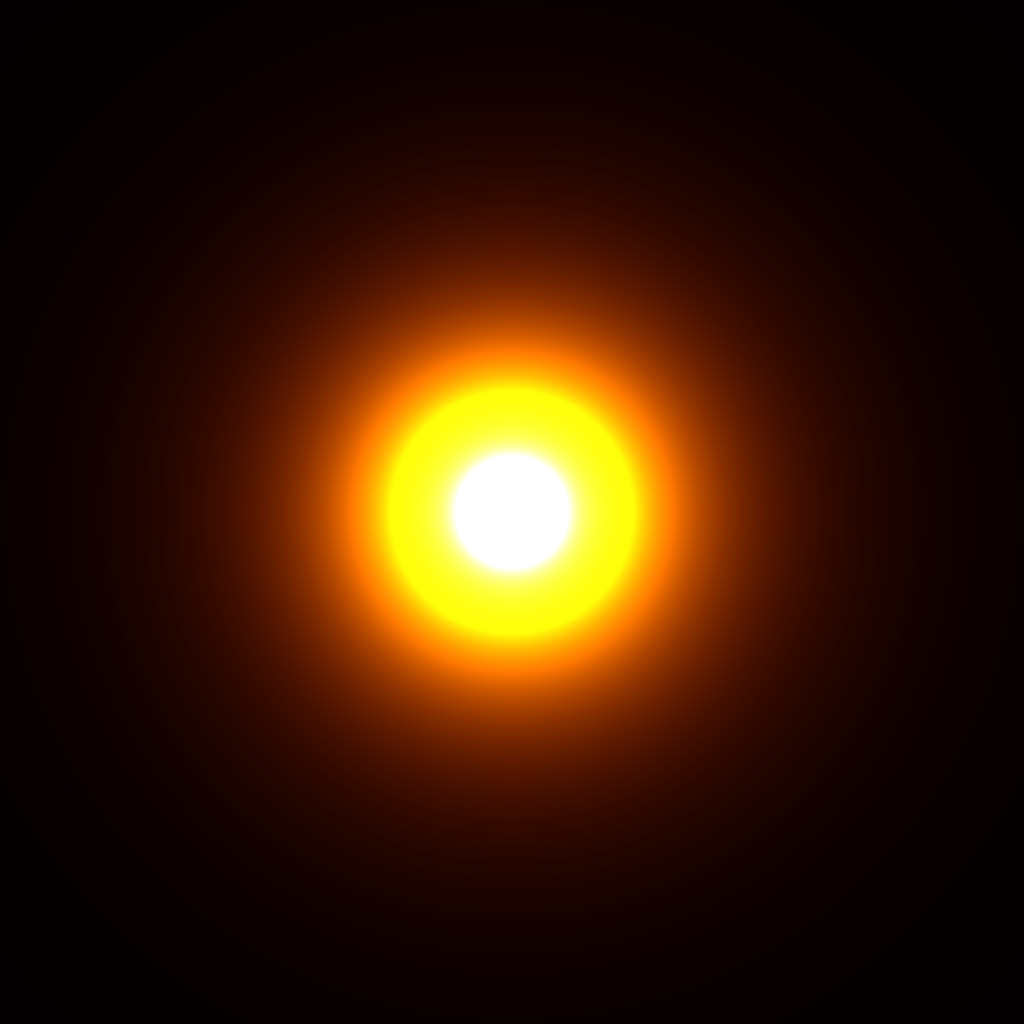
\includegraphics[width=0.8\textwidth]{images/bssrdf_slab_potato.png}
\caption{Simulation of the BSSRDF of a laser hitting a slab of 2x2 cm of potato material. We note the exponential decay of the subsurface scattering phenomena.}
\label{fig:slab_potato}
\end{figure}

In our method, in its final goal to be real time, we perform the same integral as equation \ref{eq:bssrdfeq}, but under some assumptions and restrictions that allow us to perform it more efficiently. In addition, since our method approximates the \emph{integral} and not the BSSRDF function, it is applicable to any BSSRDF function, given that it has limited or no dependence on the outgoing direction $\vomega_o$, like the directional dipole model.

The idea on approximating the integral comes from the fact that the directional dipole (and subsurface scattering effects) generally decay exponentially from the point of incidence, as we can see from figure \ref{fig:slab_potato}; where we show the simulation of a laser light hitting a surface in one point. So, the subsurface scattering contribution for points that are far apart becomes quickly negligible. The distance on which these effects become negligible is usually related to the transmission coefficient $\sigma_{tr}$. We will investigate this relation better in the result section. 

\begin{figure}
\centering
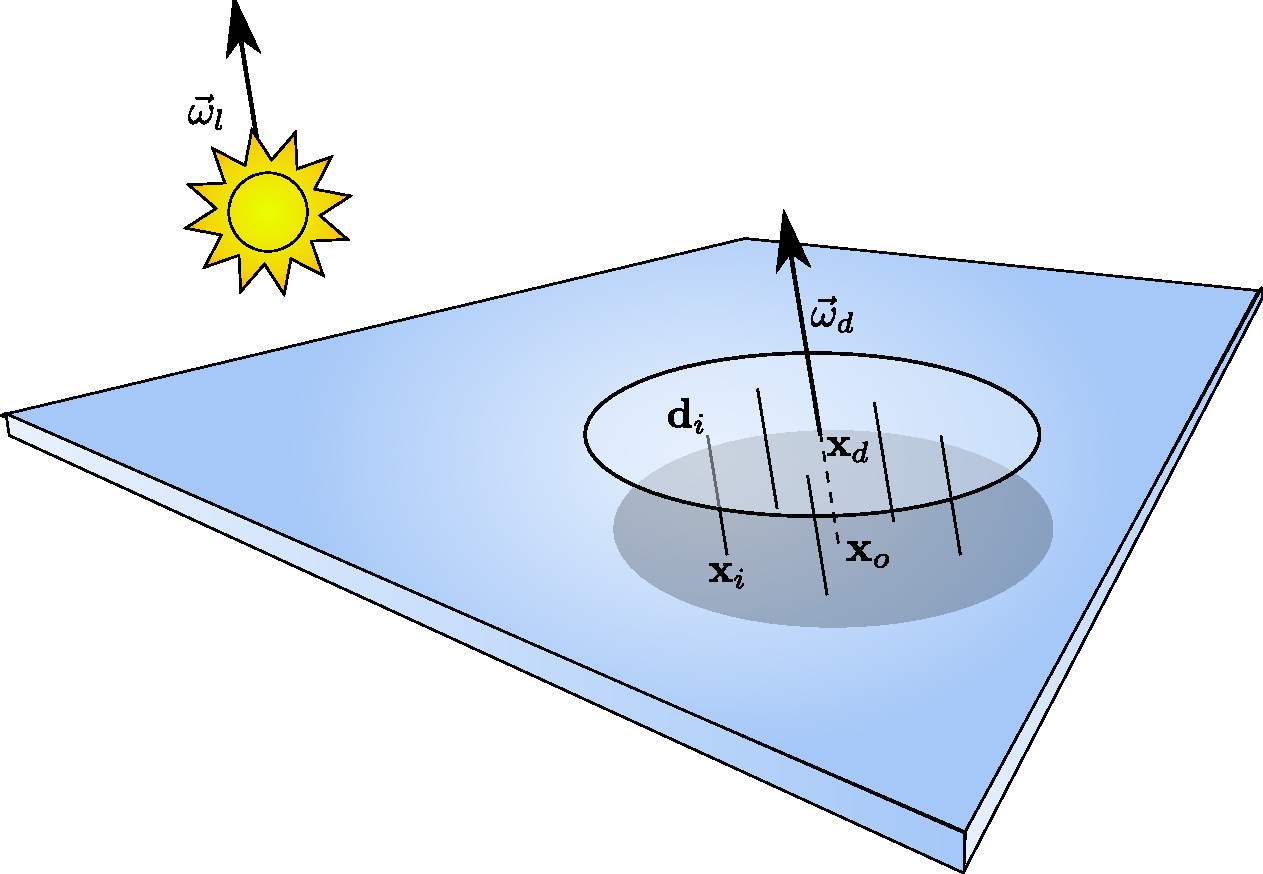
\includegraphics[width=0.8\textwidth]{images/disk_setup.pdf}
\caption{Setup for our method: the disk is placed on the point $\x_o$, displaced along the disc direction $\vomega_d$ and then the sample points $\mathbf{d}_i$ are reprojected back to find the samples $\x_i$.}
\label{fig:disksetup}
\end{figure}
\FloatBarrier

So, given this exponential decay, we place a sample disc on the surface for a position $\mathbf{x}_o$. We define a sampling disc as a point $\x_d$, a radius $r_d$ and a direction $\vomega_d$ From this disc, we chose a subset of surface points, called \emph{sample points}. To get these points, we project the points from the disc $\mathbf{d}_i$ on the surface $M$, using the disc normals as a direction (see figure \ref{fig:disksetup} for an illustration of the process). In formulas, we do:

\begin{equation*}
\x_i = \mathbf{d}_i - s \vomega_d, s \in \mathbb{R}, \x_i \in M
\end{equation*}

Then, we calculate and average the BSSRDF contribution from these points $\x_i^k$ on the point $x_o$. The process can be repeated more times for multiple lights, using the same sampling points. 

Given this set up, we need to find a way of efficiently placing the disc in order to get a good approximation of the BSSRDF. In fact, if the disc is placed in the wrong position, the accounted contribution from the sampling points will not be correct. Moreover, also the orientation of the disc is important, in order to not undersample light in certain regions of the model. A na\"{i}ve approach would suggest to pick $\x_d = \x_o$ and $\vomega_d = \vec{n}_o$, but we can see that this approach is not correct. The most obvious counter examples are displayed in Figure \ref{fig:discwrong}: in the first example \ref{fig:discwrongpoint}, the contribution from the surrounding points will be zero, because none of the sampling points is directly illuminated by the light, so the visibility term on the rendering equation will evaluate to zero. In the second example (figure \ref{fig:discwrongdir}), the wrong direction $\vec{n}_o$ prevents the most of the points from being sampled.

\begin{figure}
\centering
\subfloat[Bottom sample, na\"{i}ve approach]{
  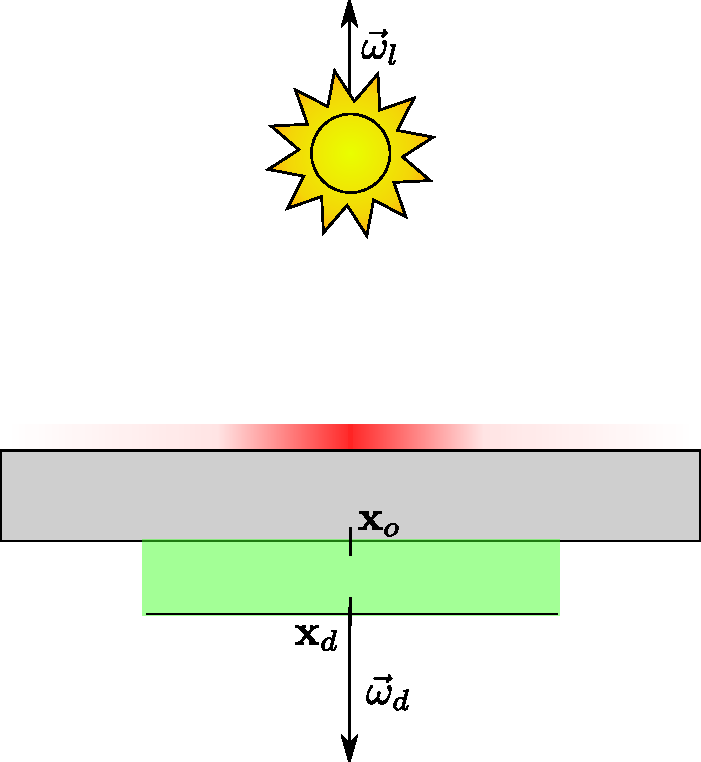
\includegraphics[width=0.5 \linewidth]{images/distribution_wrong_1.pdf}
  \label{fig:discwrongpoint}
}
\subfloat[Side sample, na\"{i}ve approach]{
  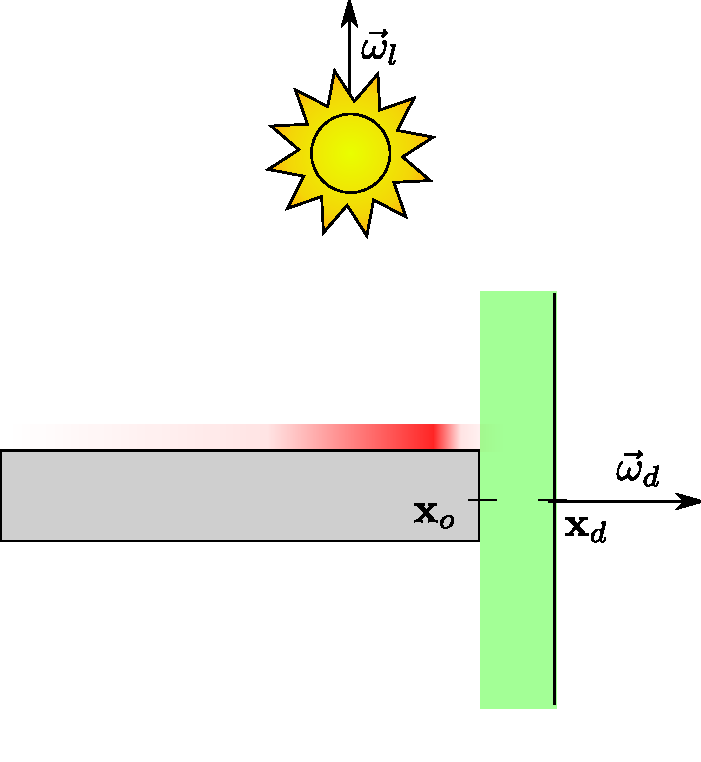
\includegraphics[width=0.5 \linewidth]{images/distribution_wrong_3.pdf}
  \label{fig:discwrongdir}
} 
\caption{Counter examples of the na\"{i}ve choice for $\x_d$ and $\vomega_d$. The green area represent the sampling area of the disc (see from the side). The red area shows where on the surface the contribution is higher for the point $\x_o$. We can see that with this approach all the contribution is actually missed.}
\label{fig:discwrong}
\end{figure}

A more careful choice for placing the points in the disc is to place the disc in a way that the obtained surface point is always the closest one to the light. To ensure that the points $\x_i$ always have this property, we can place $\x_d$ far enough from the surface in a way that all the sampling points have to be the closest to the light. If we define a \emph{bounding box vector} $\mathbb{b}$ in the same coordinate frames, we have a simple formulation for $\x_d$:

$$
\x_d = \x_o + (\mathbf{b} \cdot \vomega_l) \vomega_l
$$

The bounding box vector is a vector where its components are the maximum extension of the mesh in the coordinate reference system. So,

$$
\mathbf{b} = (\max(\x_i^x) - \min(\x_i^x), \max(\x_i^y) - \min(\x_i^y), \max(\x_i^z) - \min(\x_i^z)), \ \ \ \forall \x_i
$$ 

To solve the problem in the second example in figure \ref{fig:discwrongdir}, we chose to always orient the circle towards the light, that is $\vomega_d = \vomega_l$ for directional lights and $\vomega = \frac{\x_l - \x_d}{\|\x_l - \x_d\|}$ for point lights. As we can see, for the new choices of disc placement and orientation we are able to catch the points from where the contribution is stronger. This new setup seems much more complicated that the na\"{i}ve approach, but as we will see in the implementation section the Z-buffer of the GPU will permit us to get the desired point without any additional computation.

\begin{figure}
\centering
\subfloat[{Bottom sample, our method}]{
  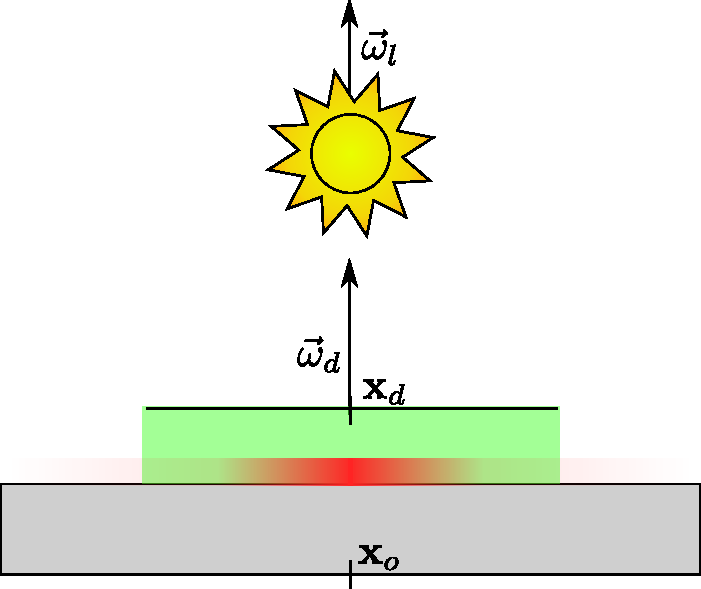
\includegraphics[width=0.5 \linewidth]{images/distribution_wrong_2.pdf}
  \label{fig:discrightpoint}
}
\subfloat[{Side sample, our method}]{
  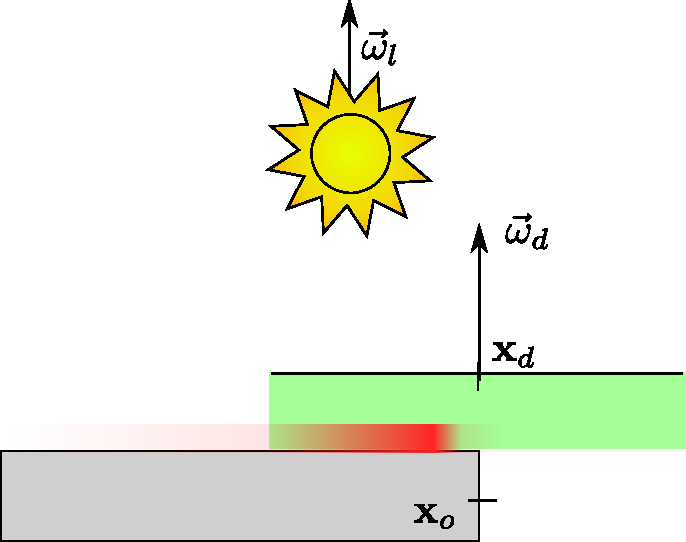
\includegraphics[width=0.5 \linewidth]{images/distribution_wrong_4.pdf}
  \label{fig:discrightdir}
} 
\label{fig:discright}
\caption{The counter examples of figure \ref{fig:discwrong} updated using our method of choice for $\x_d$. We can see that now most of the radiance distribution is accounted for.}
\end{figure}

For environment lights, we will see how to transform them in directional lights at the end of this chapter, so the setup of the equations will be the same for directional lights.

\subsection{Approximation of the rendering equation}

Going into the mathematical details the idea is to take the integral form of the rendering equation (equation \ref{eq:bssrdfeq}):

\begin{equation*}
L_o(\x_o,\vomega_o) = L_e(\x_o,\vomega_o) + \int_A \int_{2\pi} S(\x_i, \vomega_i, \x_o, \vomega_o) L_i(\x_i,\vomega_i) V(\x_i) (\vec{n}_i \cdot \vomega_i) d\vomega_i d A_i
\end{equation*}

First of all, we make the assumption of a body that is not emitting light: all the radiance from the body comes from an external source. This assumption can be trivially relaxed and implemented, but to simplify the equation in this chapter we will exclude it from the calculations. Secondly, we limit ourselves to the case of one directional light, treating the case of a point light later as an extension. The directional light direction $\vomega_l$ and radiance $L_d \ \delta(\vomega_d)$.

Under the first assumption, equation \ref{eq:bssrdfeq} becomes:

\begin{equation*}
\begin{split}
L_o^D(\x_o,\vomega_o) &= \int_A \int_{2\pi} S(\x_i, \vomega_i, \x_o, \vomega_o) L_d \ \delta(\vomega_l)\ V(\x_i) (\vec{n}_i \cdot \vomega_i) d\vomega_i d A_i \\
L_o^D(\x_o,\vomega_o) &= \int_A S(\x_i, \vomega_l, \x_o, \vomega_o) L_d  V(\x_i) (\vec{n}_i \cdot \vomega_l) d A_i 
\end{split}
\end{equation*}

In this way, we remove the internal integral. Then, in order to make a computable calculation, we need to discretize the remaining integral. We imagine to have a set of $N$ points on the surface. We assume that each one of these points is visible from the light source (so we can get rid of the $V(\x_i)$ term). We will discuss in the implementation section how to make sure that all these points are visible. Each one of these points has an associated area $A_i$, so that we can write:

\begin{equation}
L_o^D(\x_o,\vomega_o) = L_d \sum_{i = 1}^N S(\x_i, \vomega_l, \x_o, \vomega_o) (\vec{n}_i \cdot \vomega_l) A_i 
\label{eq:inter1}
\end{equation}

Now, instead of using all the points on the surface, we consider only the points within a certain radius $r^*$ from the point $\x_o$, i.e. the disk we discussed in the previous section. Assuming the points are distributed uniformly on the disk, we obtain the following area for a point:

$$
A_i = \frac{A_c}{N \ (\vec{n}_i \cdot \vomega_l)}
$$

Where $A_c = \pi (r^*)^2$ is the area of the circle. Inserting into equation \ref{eq:inter1}, we obtain:

\begin{equation}
L_o^D(\x_o,\vomega_o) = L_d \frac{A_c}{N} \sum_{i = 1}^N S(\x_i, \vomega_l, \x_o, \vomega_o)
\label{eq:inter2}
\end{equation}

That is our final approximation for a directional light. For a point light, following the exact same steps, we reach a similar solution. We recall that a point light is defined by an intensity $I_p$ and a source point $\x_p$:

\begin{equation}
L_o^P(\x_o,\vomega_o) = I_p \frac{A_c}{N} \sum_{i = 1}^N \frac{S(\x_i, \frac{\x_p - \x_i}{\|\x_p - \x_i\|}, \x_o, \vomega_o)}{\|\x_p - \x_i\|^2}
\label{eq:inter3}
\end{equation}

And, since the radiance is linearly summable, we can combine the contribution from an arbitrary number of $P_1, P_2 ... P_p$ point sources and $D_1, D_2 ... D_d$ directional sources:

\begin{equation}
\begin{split}
&L_o(\x_o,\vomega_o) = \\
&= \sum_{k=1}^{p}L_o^{P_k}(\x_o,\vomega_o) + \sum_{k=1}^{d}L_o^{D_k}(\x_o,\vomega_o) \\
&= \frac{A_c}{N} \left[ \sum_{k=1}^{p}I_p^k \sum_{i = 1}^N \frac{S(\x_i, \frac{\x_p^k - \x_i}{\|\x_p^k - \x_i\|}, \x_o, \vomega_o)}{\|\x_p^k - \x_i\|^2} + \sum_{k=1}^{d} L_d^k \sum_{i = 1}^N S(\x_i, \vomega^k_l, \x_o, \vomega_o) \right] 
\end{split}
\end{equation}


\section{Sampling patterns}
\label{sec:patterns}
As we discussed, the BSSRDF function for the directional dipole is dominated by an exponential decay. So, it is more probable to find points that contribute more to the BSSRDF if we take points closer to the evaluation point $\x_o$. However, our assumption of uniform areas in the previous calculations does not hold anymore, so we need to modify the previous equations in order to account for the non-linear sampling.

Assuming to have number generator that can generate numbers on a disc, we can create an exponentially distributed disc with the following exponential probability distribution function (PDF):

$$
pdf(x) = \sigma_{tr} e^{-\sigma_{tr} x}
$$

The difference between a disc sampled using this distribution and an uniform one is shown in figure \ref{fig:samplingweight}. The process to create this distribution will be illustrated in the implementation section, assuming for now to have already obtained one. The radius of the point $\x_i$ is: 

$$
r_i = \|\x_o^{proj} - \x_i^{proj}\|
$$

Where the two points have been projected on the circle. So now we have a new normalization term to include in order to scale back the result. So, we need now to divide by a $exp(-\sigma_{tr} r_i)$ term each sample. The new equation for a directional light then becomes:

$$
\hat{L}_o^D(\x_o,\vomega_o) = L_d \frac{A_c}{N} \sum_{i = 1}^N S(\x_i, \vomega_l, \x_o, \vomega_o) e^{\sigma_{tr} r_i}
$$

\begin{figure}
\centering
\subfloat[{Uniform sampling ($\sigma_{tr} = 1$)}]{
  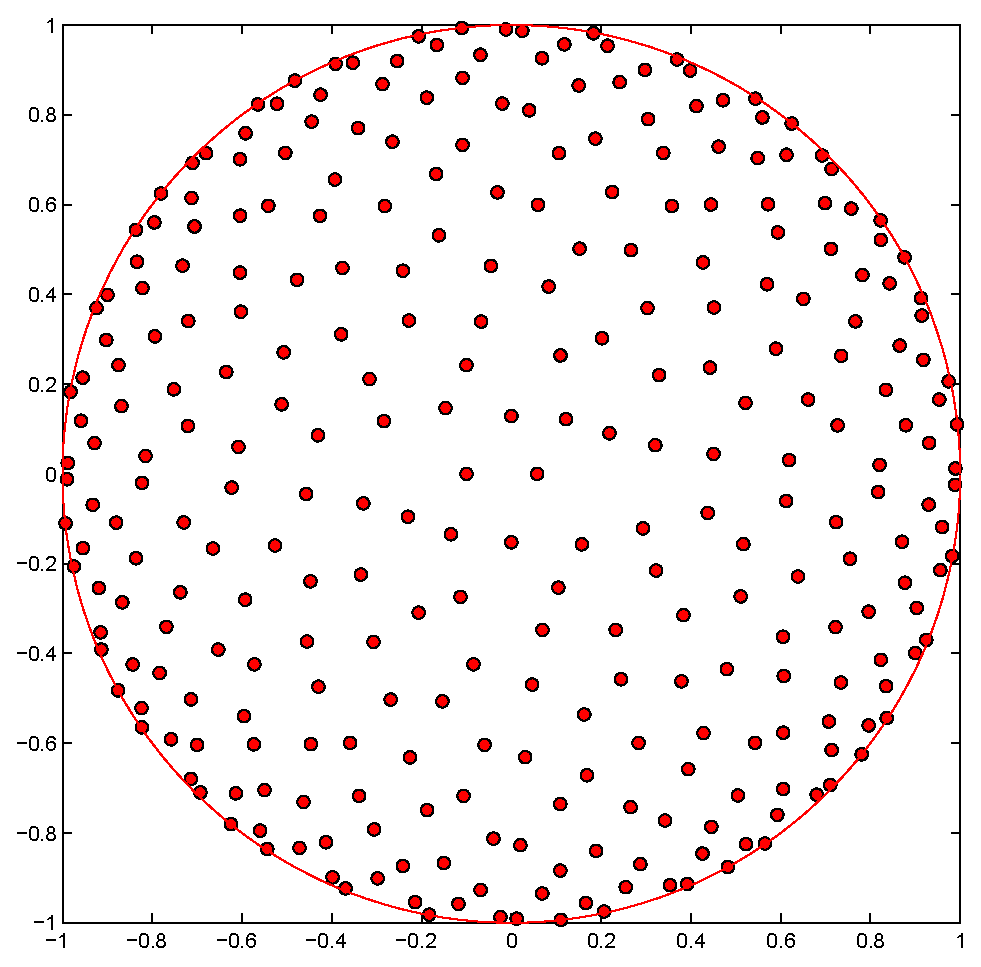
\includegraphics[width=0.5 \linewidth]{images/matlab/halton_norm.eps}
}
\subfloat[{Exponential sampling ($\sigma_{tr} = 70$)}]{
  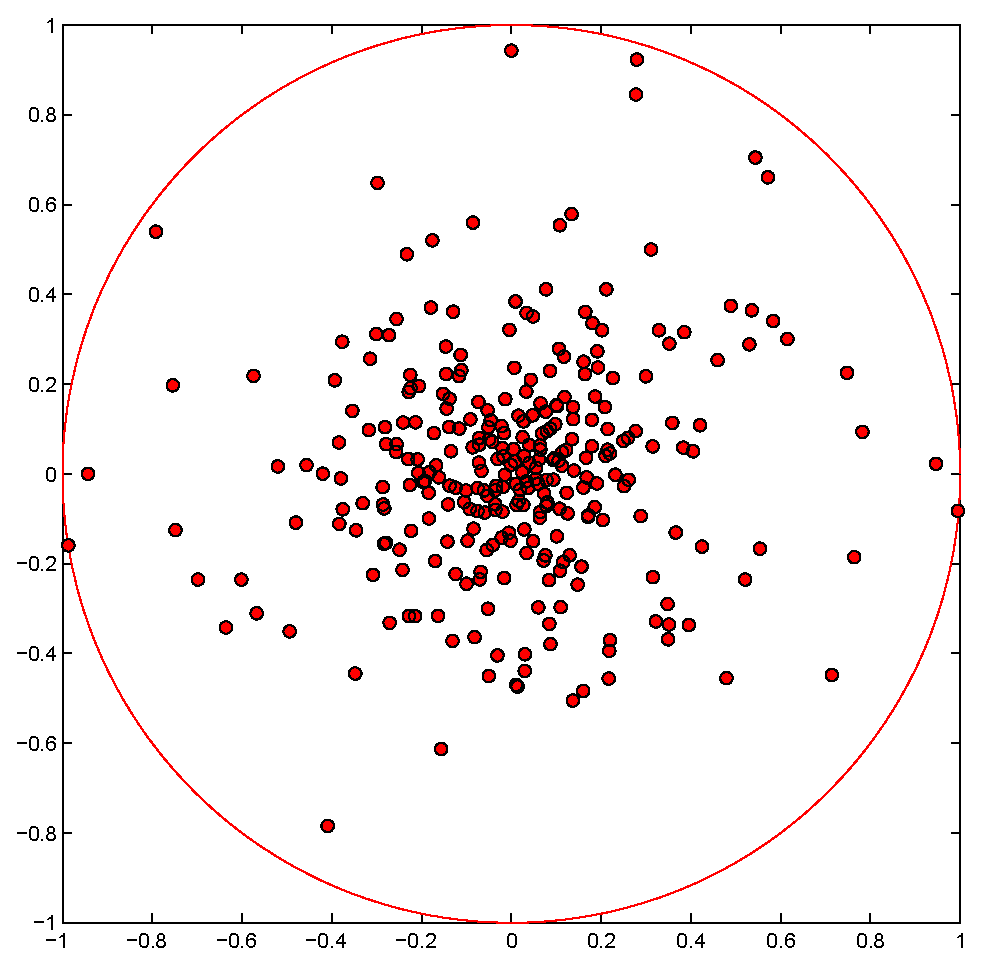
\includegraphics[width=0.5\linewidth]{images/matlab/halton_exp.eps}
} \\
\caption{Uniform versus exponentially-weighted sampling of 300 points.}
\label{fig:samplingweight}
\end{figure}

The other two equations \ref{eq:inter2} and \ref{eq:inter2} then change accordingly:

$$
\hat{L}_o^P(\x_o,\vomega_o) = I_p \frac{A_c}{N} \sum_{i = 1}^N \frac{S(\x_i, \frac{\x_p - \x_i}{\|\x_p - \x_i\|}, \x_o, \vomega_o)}{\|\x_p - \x_i\|^2}  e^{\sigma_{tr} r_i}
$$

\begin{equation*}
\begin{split}
&\hat{L}_o(\x_o,\vomega_o) = \\
&= \sum_{k=1}^{p}\hat{L}_o^{P_k}(\x_o,\vomega_o) + \sum_{k=1}^{d}\hat{L}_o^{D_k}(\x_o,\vomega_o) \\
&= \frac{A_c}{N} \left[ \sum_{k=1}^{p}I_p^k \sum_{i = 1}^N \frac{S(\x_i, \frac{\x_p^k - \x_i}{\|\x_p^k - \x_i\|}, \x_o, \vomega_o)}{\|\x_p^k - \x_i\|^2} e^{\sigma_{tr} r_i} + \sum_{k=1}^{d} L_d^k \sum_{i = 1}^N S(\x_i, \vomega^k_l, \x_o, \vomega_o) e^{\sigma_{tr} r_i}\right] 
\end{split}
\end{equation*}

\section{Parameter acquisition}
When rendering translucent materials, it is important that we have the right scattering properties, in order to match the appearance of real world objects. The scattering parameters may be tweaked by the artist and set up manually, but this is a long process since the the scattering properties are not directly related to material appearance. In order to avoid this problems, the scattering parameters are measured from samples taken from real world objects. In this section, we will give an overview of two methods used to estimate the scattering parameters.

The first method was presented alongside the standard dipole model by \cite{Jensen:2001:PMS:383259.383319}. The measurement apparatus consists of a series of lenses that focus the light on the sample. The light power $\Phi$ is measured by calibrating the sensor with a spectralon sample. A picture of the sample is then acquired at different exposure, in order to build an high dynamic range image. This is necessary since the scattering decays exponentially, so a high range is needed to have meaningful measurements. The measured data are then fitted to diffusion theory in order to obtain the scattering coefficients. Due to the nature of the measurement, it is not possible to measure the mean cosine $g$ of the material, but only the reduced scattering coefficient $\sigma_s' = \sigma_s (1 - g)$ and the absorption coefficient $\sigma_a$. This measurement model uses the diffusion approximation to work, so it shares the same limitations: it is valid only for materials where $\sigma_a \ll \sigma_s$.

The second method, proposed by \cite{Narasimhan:2006:ASP:1141911.1141986} proposes a method to measure the scattering coefficient by dilution. The assumption is that water does not interfere with the scattering properties of the materials dissolved within it for small distances (less than \SI{50}{cm}). Naturally, the material needs then to be already in  a liquid form, or to be a powder that can be easily dissolved in water. The setup of the experiment is a box full of water with a camera and an area light. High dynamic range picture of the material dissolved in water are then taken, and the scattering coefficients can be measured with a low error. Various measurements at different concentrations are needed in order to get an effective measurement of the coefficients, but then the coefficients can be extrapolated for any concentration. 

Some of the scattering properties measured thanks to this method are reported in table \ref{table:scatteringcoefficients}. This coefficients will be used throughout the report when referencing to a specific material.
\clearpage
\begin{landscape}
\renewcommand{\arraystretch}{1.8}
\begin{table}[!ht]
    \centering
    \begin{tabular}{|l|ccc|ccc|ccc|c|c|}
    \hline
    \multirow{2}{*}{Material}               & \multicolumn{3}{|c|}{Absorption, $\sigma_a$}     & \multicolumn{3}{|c|}{Scattering, $\sigma_s$}     & \multicolumn{3}{|c|}{Mean cosine, $g$}    & \multirow{2}{*}{$\eta$} & \multirow{2}{*}{Source} \\ 
               &R& G      & B     & R & G      & B      & R   & G     & B     &  &  \\ \hline
    {Apple}                  & 0.0030 & 0.0034 & 0.0046 & 2.29   & 2.39   & 1.97   & -     & -     & -     & 1.3    & J      \\
    {Ketchup}                & 0.061  & 0.97   & 1.45   & 0.18   & 0.07   & 0.03   & -     & -     & -     & 1.3    & J      \\
    {Marble}                 & 0.0021 & 0.0041 & 0.0071 & 2.19   & 2.62   & 3.00   & -     & -     & -     & 1.5    & J      \\
    {Potato}                 & 0.0024 & 0.0090 & 0.12   & 0.68   & 0.70   & 0.55   & -     & -     & -     & 1.3    & J      \\
    {Whole milk}             & 0.0011 & 0.0024 & 0.014  & 2.55   & 3.21   & 3.77   & -     & -     & -     & 1.3    & J      \\
    {Coffee}                 & 0.1669 & 0.2287 & 0.3078 & 0.2707 & 0.2828 & 0.297  & 0.907 & 0.896 & 0.88  & 1.3    & N    \\
    {Soy milk}               & 0.0001 & 0.0005 & 0.0034 & 0.2433 & 0.2714 & 0.4563 & 0.873 & 0.858 & 0.832 & 1.3    & N      \\
    {Wine (merlot)   }       & 0.7586 & 1.6429 & 1.9196 & 0.0053 & 0      & 0      & 0.974 & 0     & 0     & 1.3    & N      \\
    {Beer (Budweiser)}       & 0.1449 & 0.3141 & 0.7286 & 0.0037 & 0.0069 & 0.0074 & 0.917 & 0.956 & 0.982 & 1.3    & N      \\
    {White grapefruit juice} & 0.0096 & 0.0131 & 0.0395 & 0.3513 & 0.3669 & 0.5237 & 0.548 & 0.545 & 0.565 & 1.3    & N      \\ \hline
    \end{tabular}
		\caption{Scattering material parameters estimated using different methods. For the source field, \texttt{J} materials come from \cite{Jensen:2001:PMS:383259.383319}, while \texttt{N} materials come from \cite{Narasimhan:2006:ASP:1141911.1141986}. Note that the materials measured with the technique proposed in \cite{Jensen:2001:PMS:383259.383319} are without the $g$ coefficient.}
		\label{table:scatteringcoefficients}
\end{table}
\end{landscape}
\clearpage

\begin{figure}
\centering
\subfloat[Apple]{
  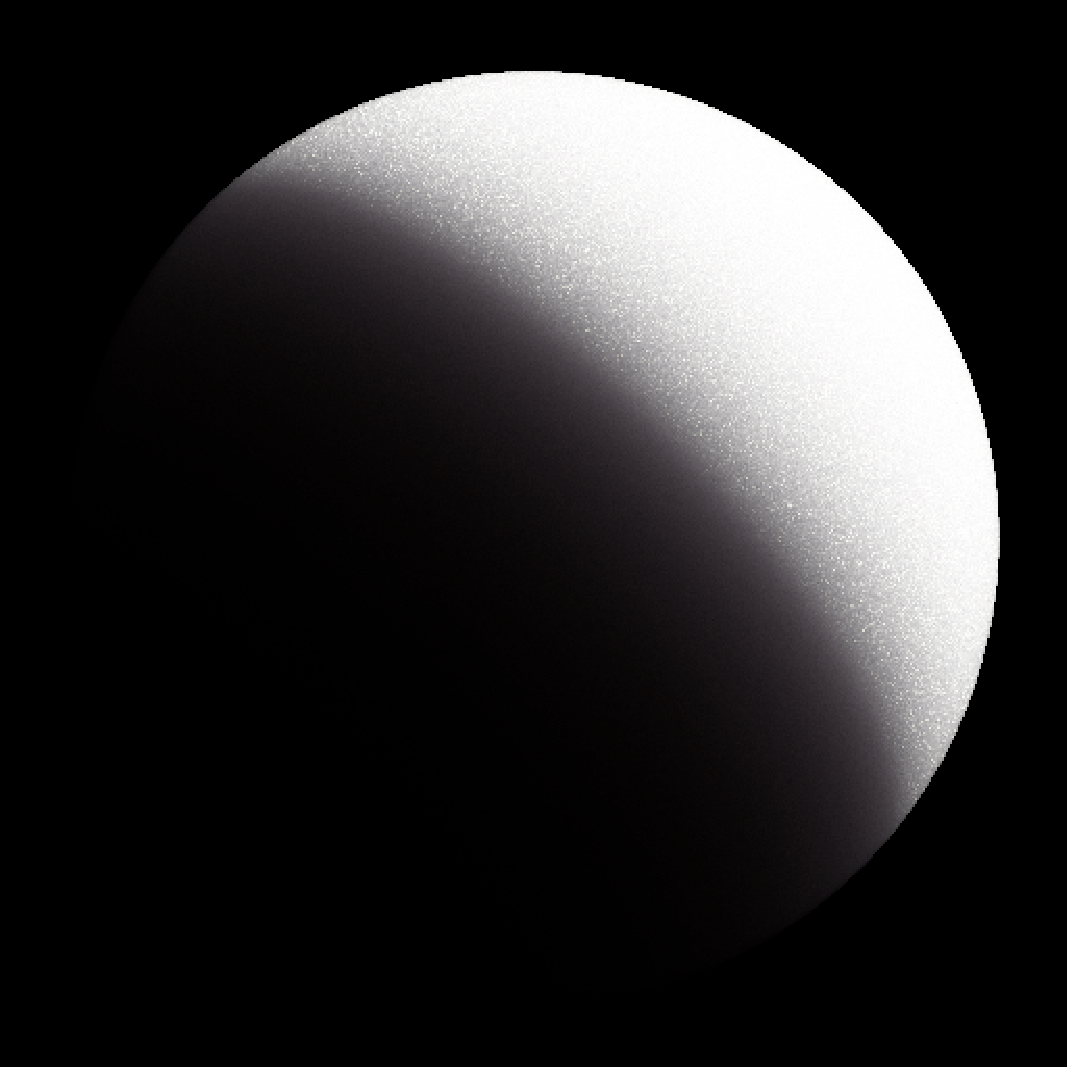
\includegraphics[width=0.33 \linewidth]{images/pathtrace/image-apple.pdf}
}
\subfloat[Marble]{
  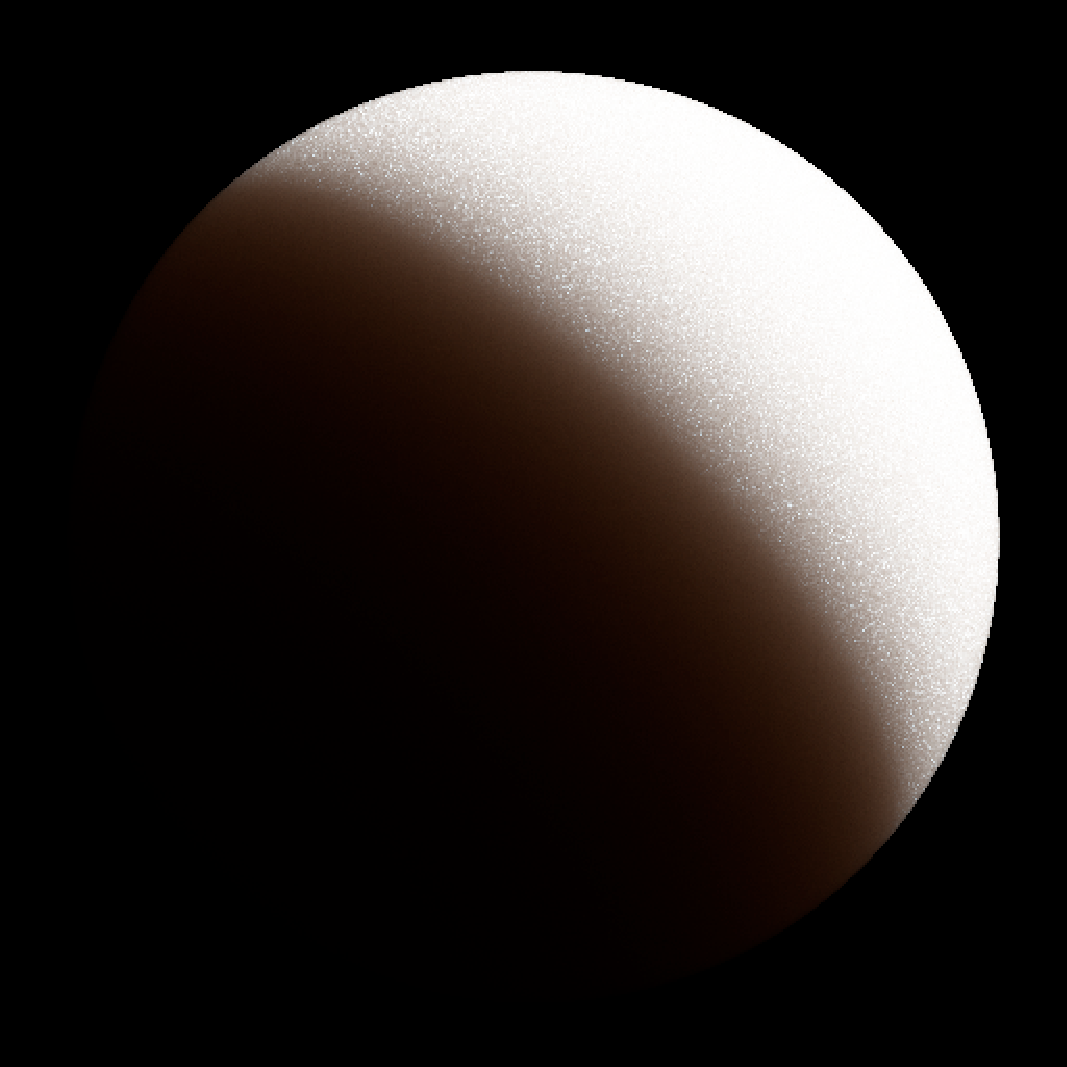
\includegraphics[width=0.33 \linewidth]{images/pathtrace/image-marble.pdf}
}
\subfloat[Potato]{
  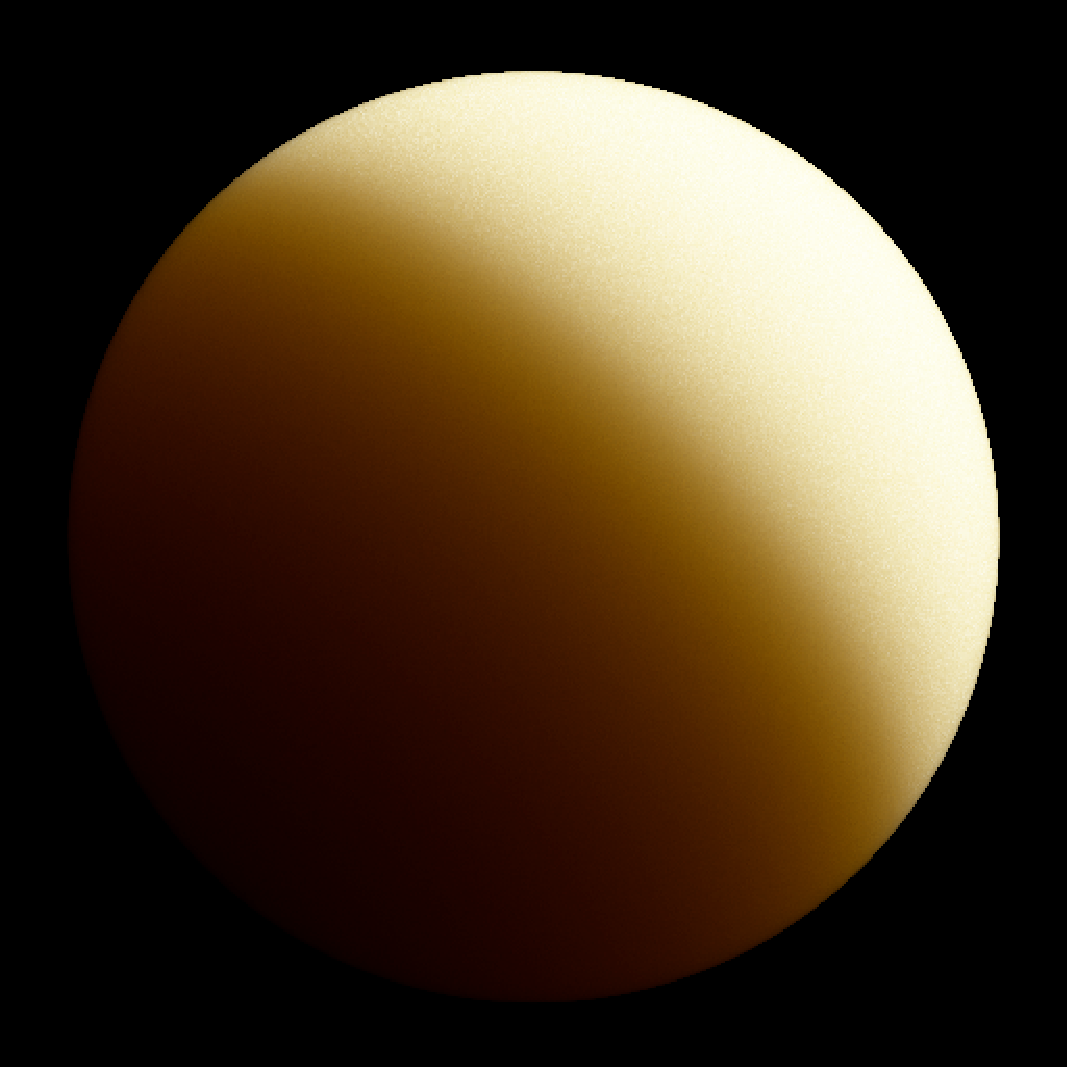
\includegraphics[width=0.33 \linewidth]{images/pathtrace/image-potato.pdf}
} \\
\subfloat[Whole Milk]{
  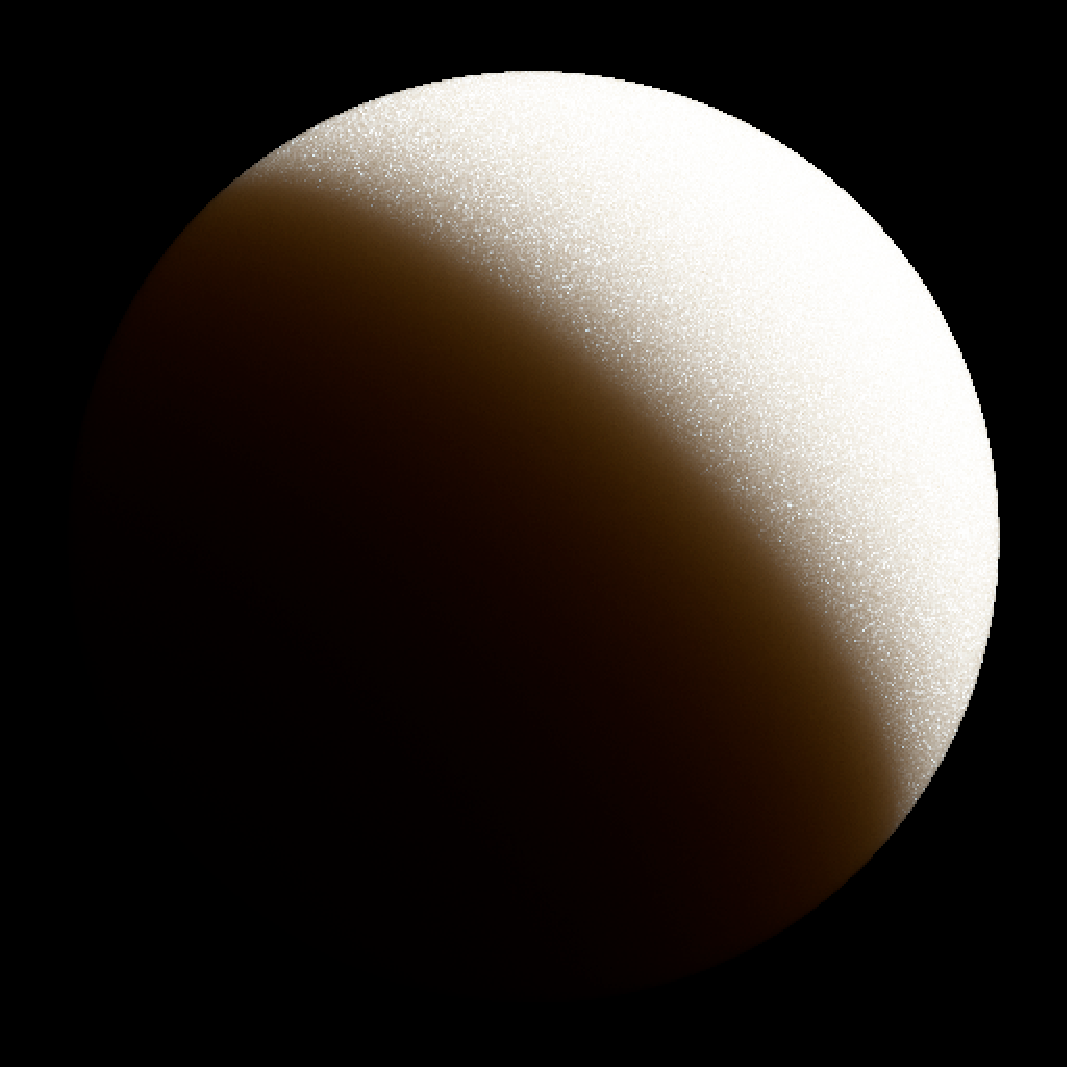
\includegraphics[width=0.33 \linewidth]{images/pathtrace/image-wholemilk.pdf}
}
\subfloat[Coffee]{
  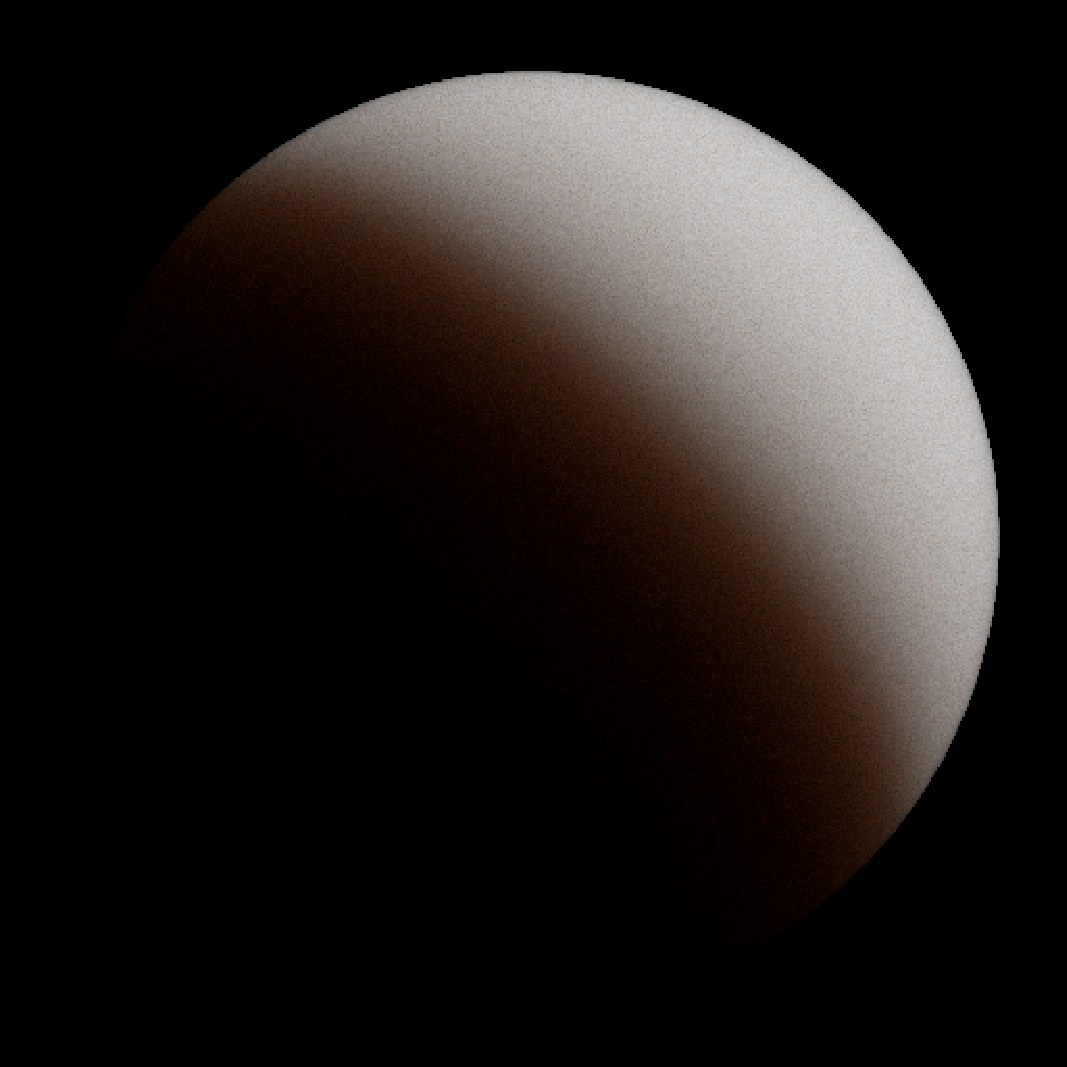
\includegraphics[width=0.33 \linewidth]{images/pathtrace/image-coffee.pdf}
}
\subfloat[Soy Milk]{
  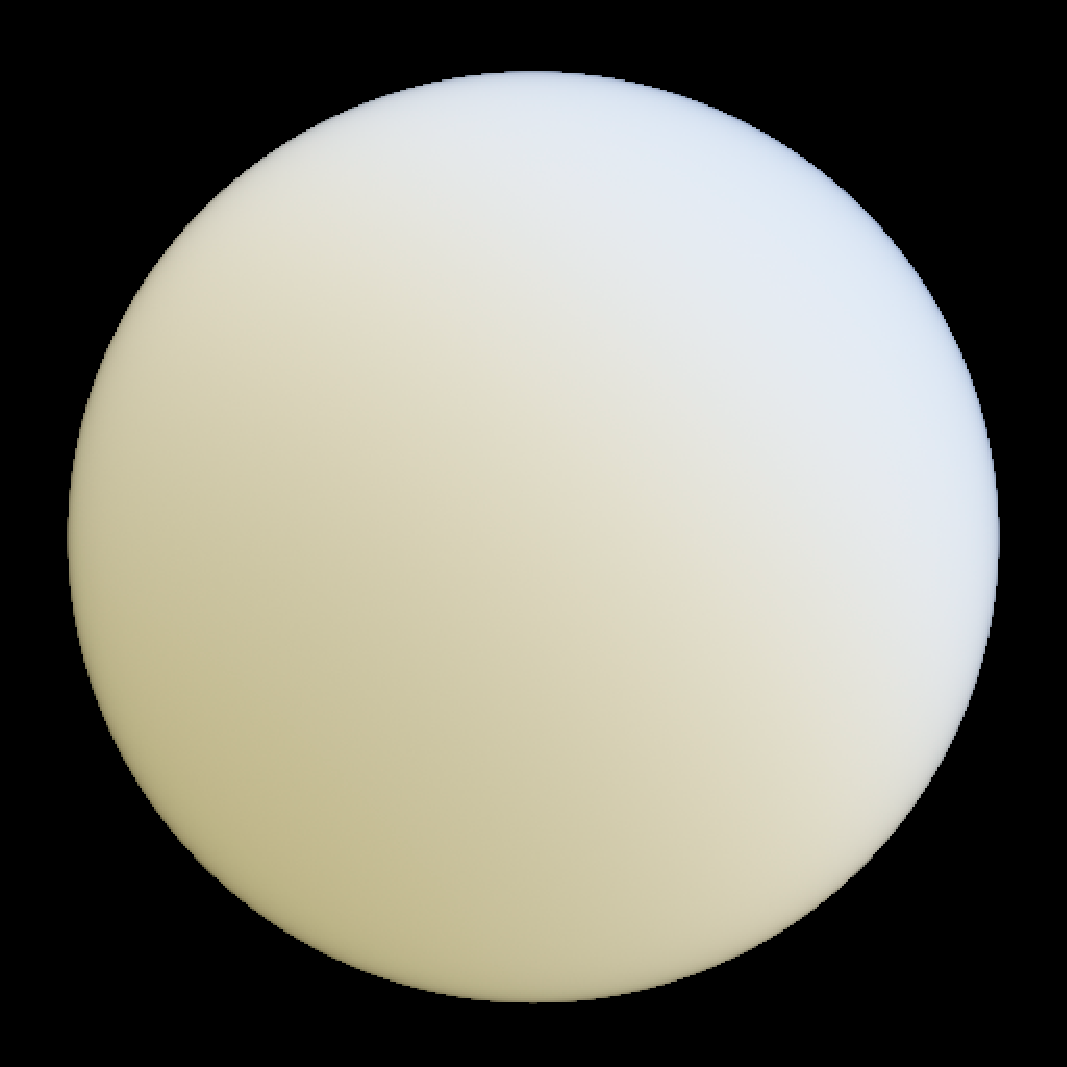
\includegraphics[width=0.33 \linewidth]{images/pathtrace/image-soymilk.pdf}
} \\
\subfloat[Wine (merlot)]{
  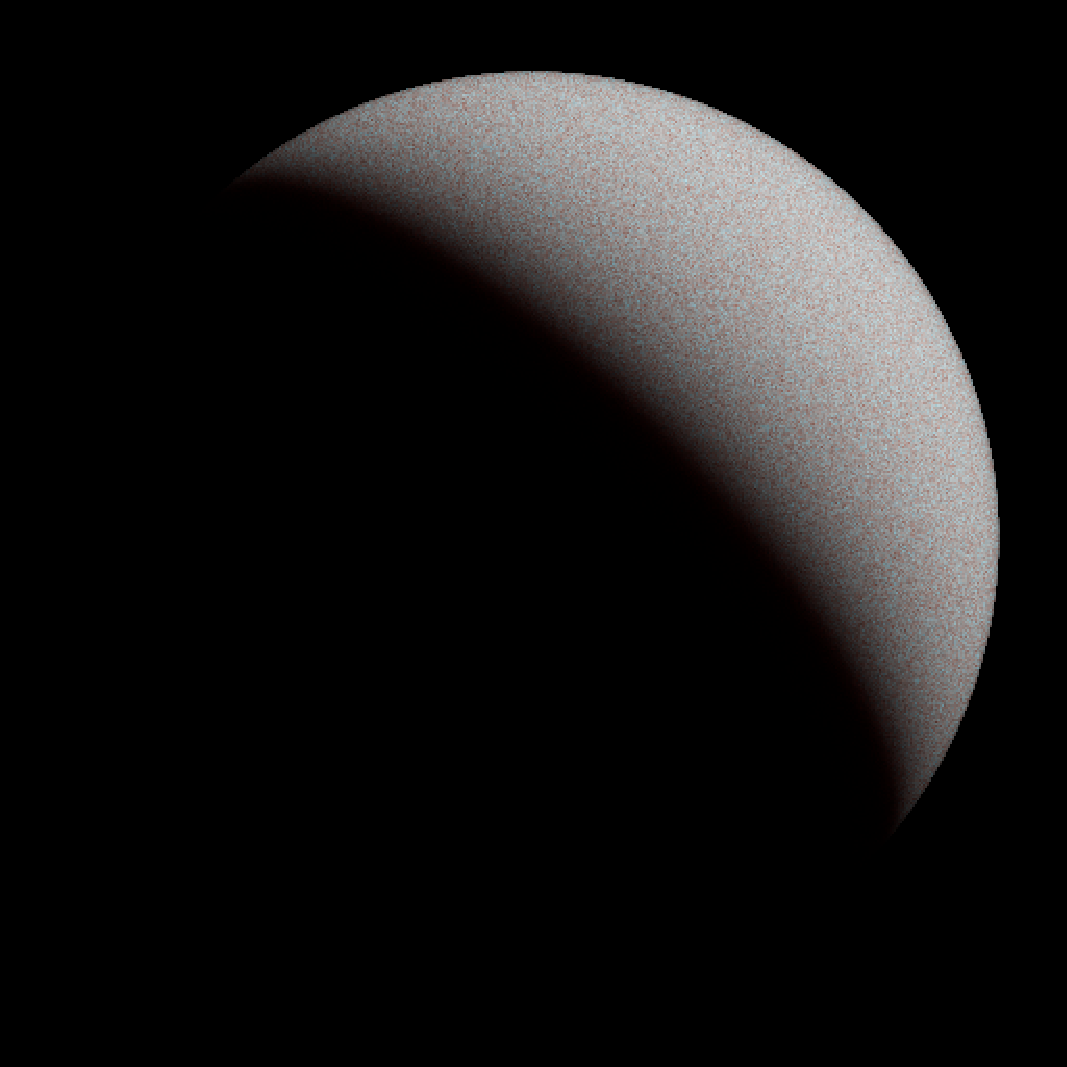
\includegraphics[width=0.33 \linewidth]{images/pathtrace/image-merlot.pdf}
}
\subfloat[Beer (Budweiser)]{
  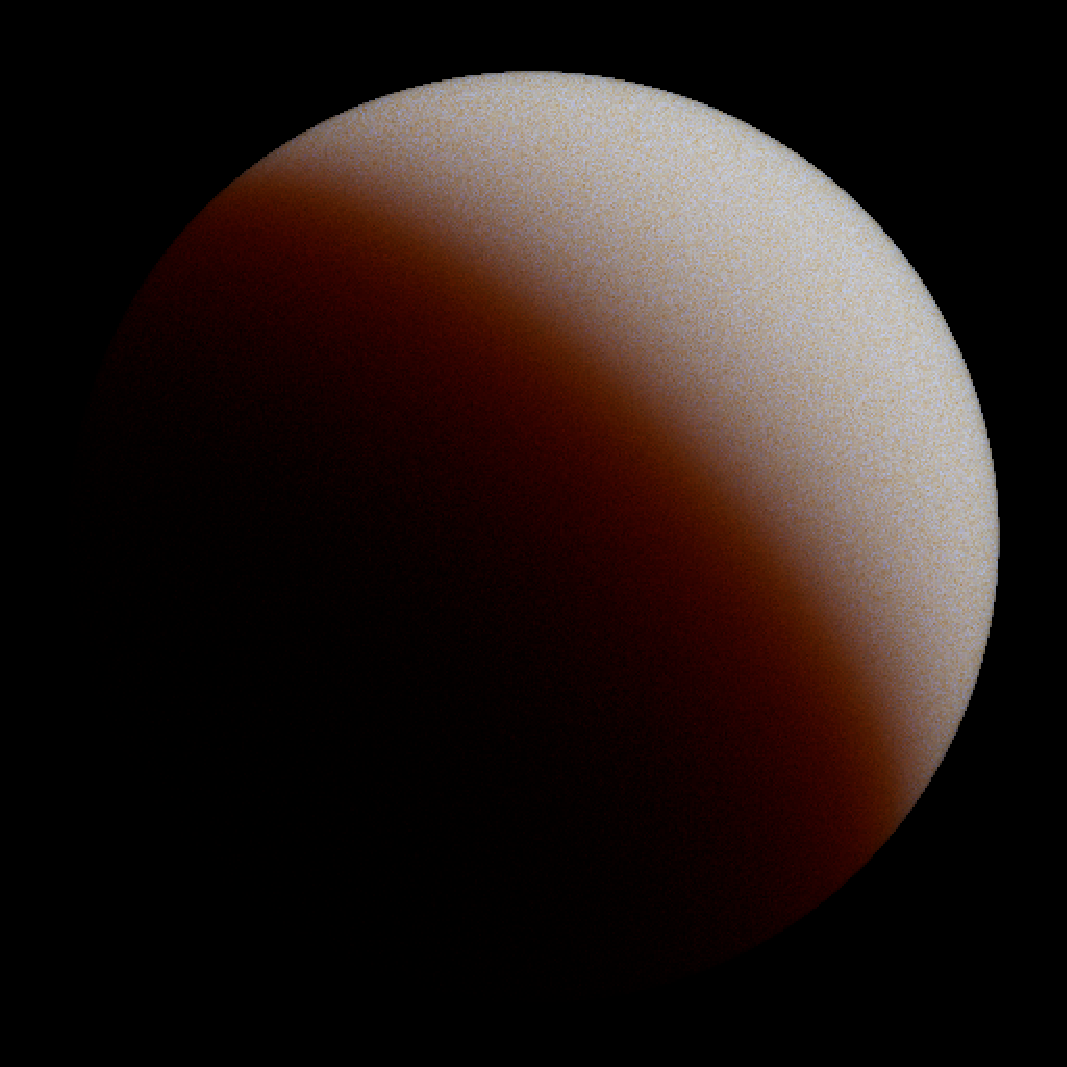
\includegraphics[width=0.33 \linewidth]{images/pathtrace/image-beer.pdf}
}
\subfloat[White Grapefruit Juice]{
  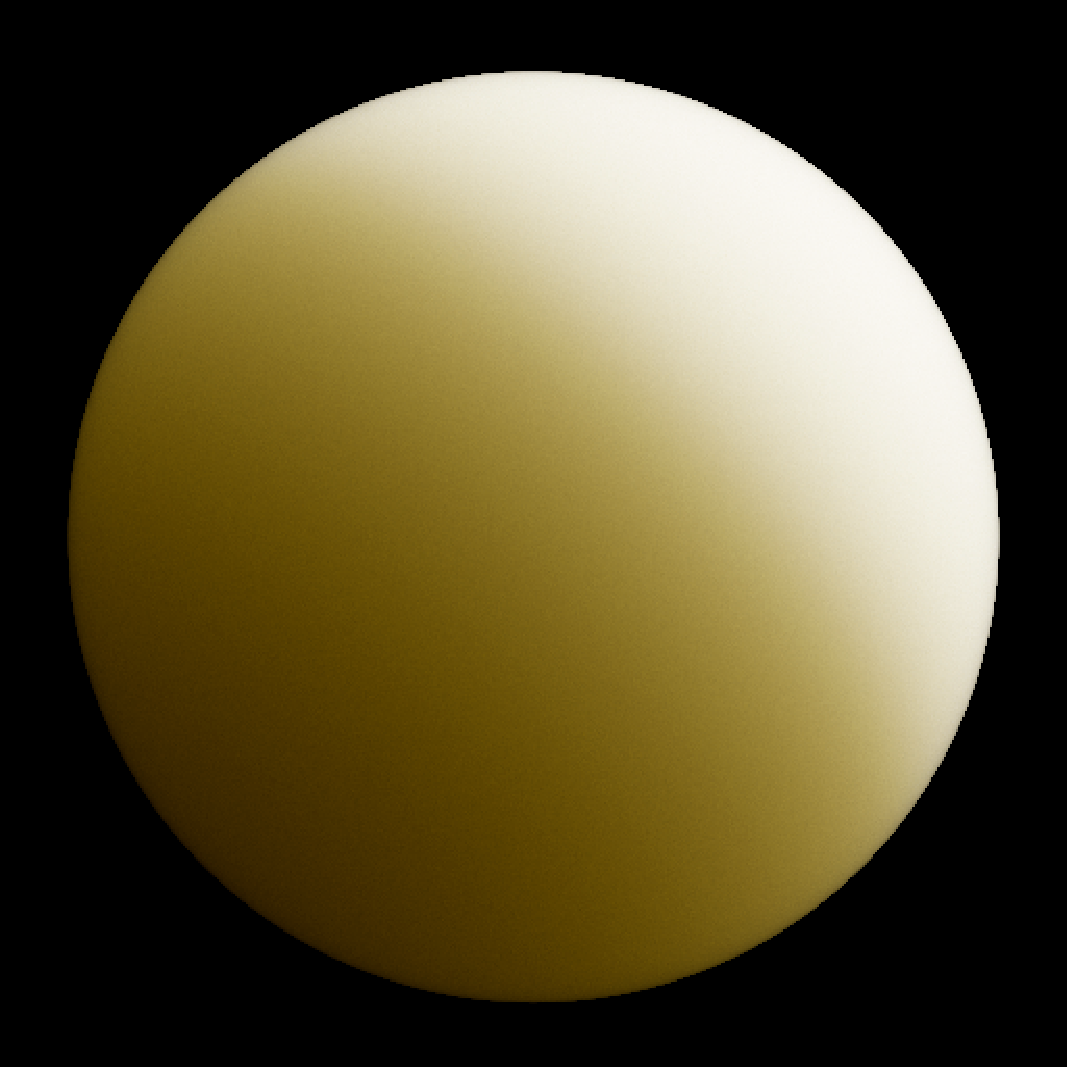
\includegraphics[width=0.33 \linewidth]{images/pathtrace/image-grapefruit.pdf}
} \\
\label{fig:examplesmaterials}
\caption{Path traced rendering on a sphere of the materials described in table \ref{table:scatteringcoefficients}.}
\end{figure}
\clearpage

\section{Environment lights}
\label{sec:env}
Environment lighting is a omni-directional lighting that represents lighting coming from an environment. Instead of defining a light as a direction or a point in space, we define directly the radiance distribution on a map. The map is usually provided in a HDR format in order to cover various range of radiance, and it is usually given as a set of six cube faces (cubemap) or as a latitude-longitude map, as the one in figure \ref{fig:doge}. The maps are usually given in equirectangular projection.

In the game development community, spherical harmonics (SH) \citep{green,peterpikeconference} are usually employed. This technique, given an heavy pre-computation step, transforms the radiance map into a set of coefficients in the spherical harmonics basis. This coefficients that then can be used easily to represent the radiance map, if we are interested only in the low-frequency part of it. 

\begin{figure}[!ht]
\centering
\includegraphics[width=\textwidth]{images/matlab/doge2.png}
\caption{Latitude - longitude environment map of the inner courtyard of the Doge's palace in Venice (Doge map). The map has been converted to a RGB format from the original HDR format. Image courtesy of \url{http://gl.ict.usc.edu/Data/HighResProbes/}.}
\label{fig:doge}
\end{figure}

In this chapter, we introduce a technique presented in \cite{Pharr:2004:PBR:975275} to convert a environment map into a set of directional light sources of arbitrary size. The general idea is to generate a set of random points and them transform them according to a pre-computed probability distribution. This distribution make the random point concentrate in areas where the radiance is higher, so that it is possible to get the most representative points on the radiance map. The found points are then transformed into a spherical coordinate basis in order to get the light direction.

We start defining our image as an array of $n$ rows and $m$ columns. We need to define a function that of each pixel of the image gives us a single radiance value. Instead of using radiance, we use luminance. The ITU-R recommendation standard BT.709\citep{BT.709-2} gives us a formula to obtain luminance from spectral radiance values:

$$
f(u,v) = 0.2126\ R(u,v) + 0.7152\ G(u,v) + 0.0722\ B(u,v)
$$

Where $[u,v] \in [0,n)\times [0,m)$. $R$, $G$ and $B$ represent the spectral coordinates of the radiance map. We would like to define now a probability distribution function based on the $f(u,v)$ function. We can define it simply by normalizing $f$ with the integral of the function over the domain:

$$
p(u,v) = \frac{f(u,v)}{ \displaystyle\iint f(u,v) du dv} = \frac{f(u,v)}{ \displaystyle\sum_u \sum_v f(u,v)}
$$

However, in order to be able to sample from the distribution $p(u,v)$, there are some things to take care about. We would like now to separate the two variables, in order to sample from two one-dimensional distribution, instead of one two-dimensional distribution. To do this, we use the conditional probability formula:

$$
p(u,v) = p_v(v|u) p_u(u)
\label{eq:conditional_prob}
$$

So that we first choose u, sample its probability $p_u(u)$ and then compute the conditional density $p_v(v|u)$ using the found value for $u$. Using the marginal formulas, the first probability is easily found:

$$
p_u(u) =\int p(u,v) dv = \frac{ \displaystyle\sum_v f(u,v)}{ \displaystyle\sum_u \sum_v f(u,v)}
$$

And, from equation \ref{eq:conditional_prob}, we find the conditional probability:

$$
p_v(v|u) = \frac{p(u,v)}{p_u(u)} = \frac{f(u,v)}{ \displaystyle\sum_v f(u,v)} \sin \theta
$$

The $\sin \theta$ comes from the fact that the latitude-longitude map with a equirectangular projection is not area preserving. So, the sampling must take into account the distortion of the map, otherwise the samples will be more concentrated at the poles, rather than distributed uniformly on the sphere. We can appreciate the difference for a random sampling on a sphere in figure \ref{fig:randomsamplingsphere}.

\begin{figure}[!ht]
\centering
\subfloat[Without $\sin\theta$ correction]{
  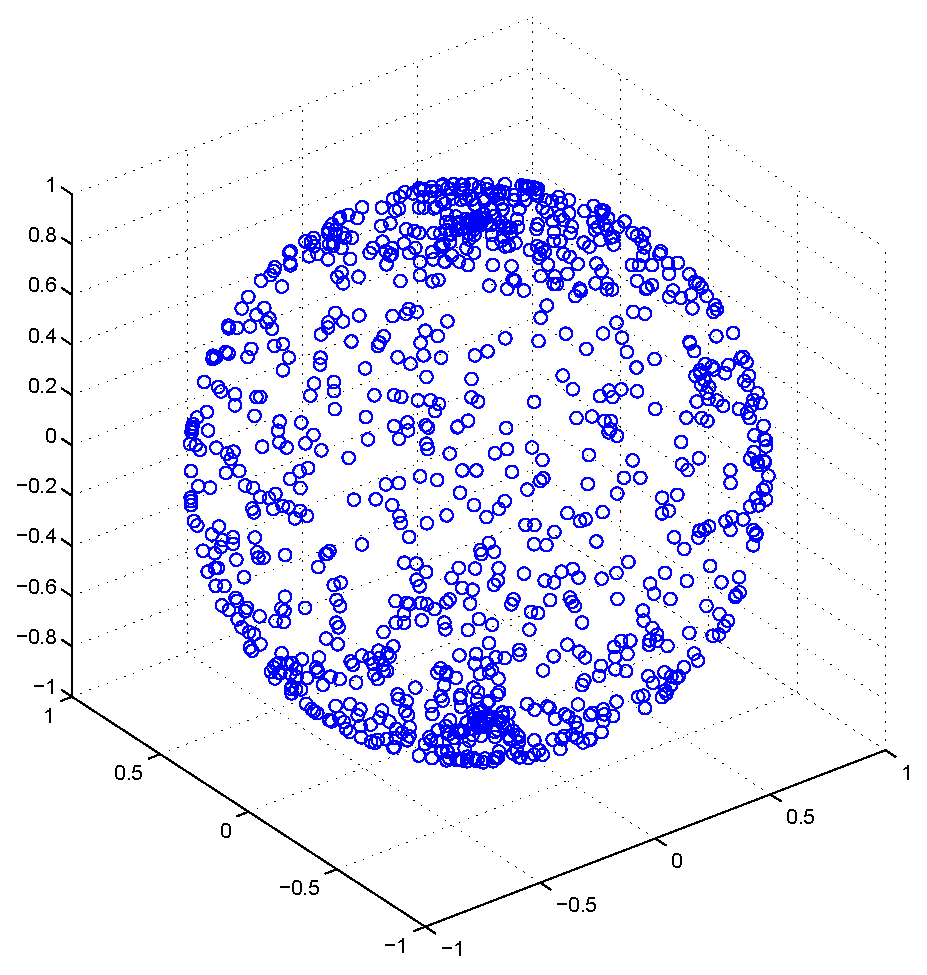
\includegraphics[width=0.5 \linewidth]{images/matlab/notunif.eps}
}
\subfloat[With $\sin\theta$ correction]{
  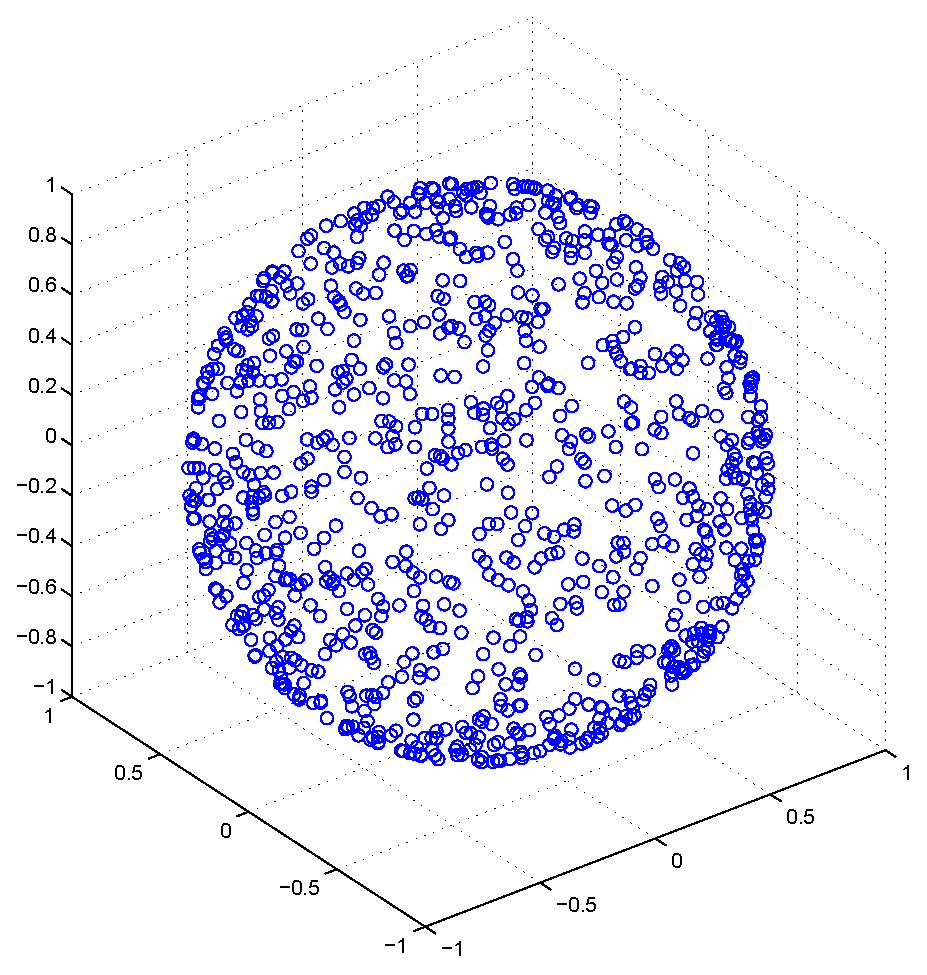
\includegraphics[width=0.5\linewidth]{images/matlab/unif.eps}
} \\
\caption{Effect of $\sin\theta$ on a random point distribution on a sphere.}
\label{fig:randomsamplingsphere}
\end{figure}

Now we are ready to sample the function. In order to bias our sample according to the radiance distribution, we need to calculate the cumulative distribution function (CDF) for a one-dimensional probability distribution function. The CDF is defined as:

$$
c_u(u) = \int_{-\infty}^{u} p_u(u) du = \sum_{i=0}^u p_u(u)
$$

That is the discrete integral of the function up to the point $u$. Figure \ref{fig:cdfweight} explain why. If, as the figure, all the radiance is distributed towards the right side of the picture (i.e. the CDF rises slowly), if we pick a set of random points and reverse the CDF on them, we obtain a new set of points that is biased towards the highest concentration of radiance.

%\begin{figure}
%\centering
%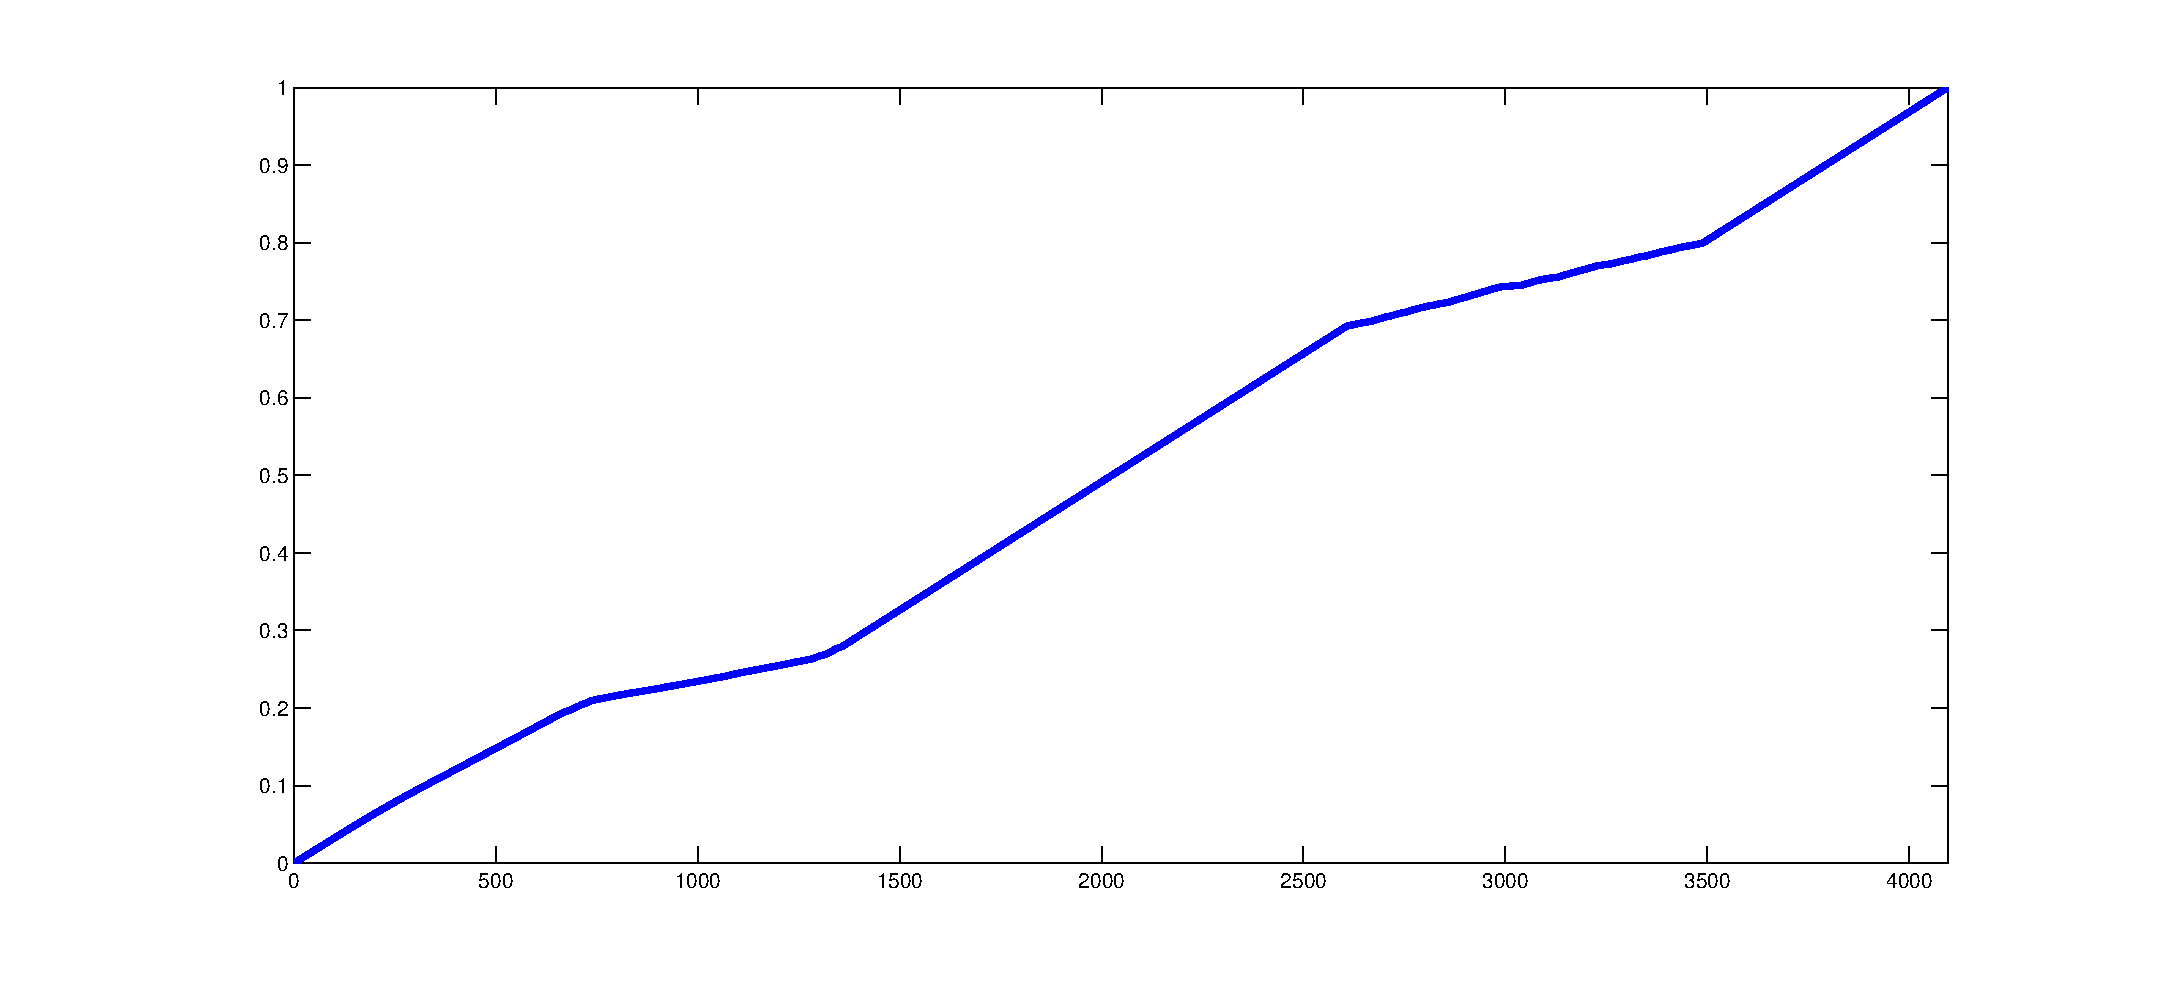
\includegraphics[width=\textwidth]{images/matlab/doge_green_line.eps}
%\caption{CDF for luminance of line 450 of the doge skybox.}
%\label{fig:cdf}
%\end{figure}

\begin{figure}[!ht]
\centering
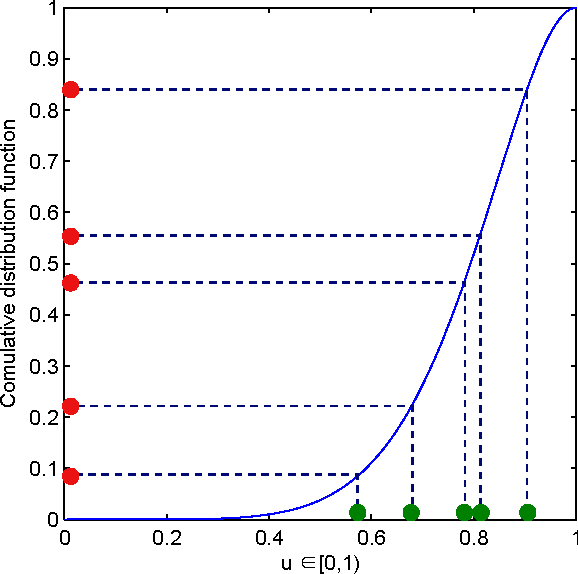
\includegraphics[width=0.5\textwidth]{images/matlab/cdfex.pdf}
\caption{Effect of weighting values with the CDF. We note that the random values on the $y$ axis are transformed and accumulated where the CDF is steeper.}
\label{fig:cdfweight}
\end{figure}

Let us now pick a couple of random points $(\zeta_1,\zeta_2) \in [0,1)^2$. We then convert these points to a pair of coordinates $(u_1,u_2) \in [0,n)\times[0,m)$ by inverse sampling of the CDF. We will give the details of how to discretize this process in the implementation section. Then, we obtain the spherical coordinates using the standard formula:

$$
(\theta, \phi) = \left(\frac{u_1}{\pi n}, \frac{u_2}{2 \pi m}\right)
$$

And, from the spherical coordinates, we use the equirectangular projection formula to transform them into a vector in the 3D space, that is the final direction for our light.

$$
\vomega_l = (\cos\phi\;\sin\theta, \sin\phi\;\sin\theta, \cos\theta)
$$

And, by varying the random values $(\zeta_1,\zeta_2)$, obtain a set of directions that we can use for rendering. The generated points for the Doge map can be seen in figure \ref{fig:doge_lights}.


\begin{figure}
\centering
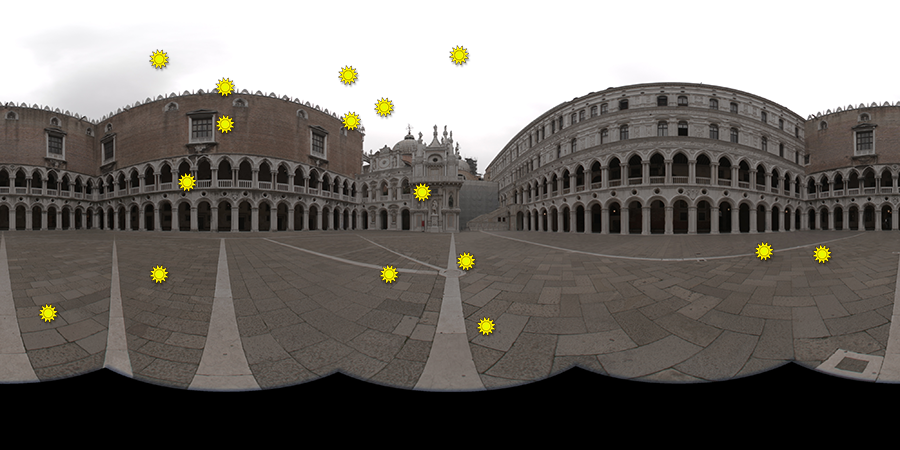
\includegraphics[width=\textwidth]{images/matlab/doge2_lights.png}
\caption{Position of calculated lights for the doge map.}
\label{fig:doge_lights}
\end{figure}